\chapter{REVISIÓN CRÍTICA DE LA LITERATURA}

Para desarrollar un sistema tecnológico se debe conocer qué existe actualmente en el mercado, tanto en hardware como en software. En este sentido, se buscará entre las distintas empresas qué servicios realizan para las granjas de jaula, qué robots utilizan y qué métodos utilizan relacionados la visión computacional. Seguidamente, con el fin de simular correctamente el sistema desarrollado, se debe identificar qué software de simulación es el mejor para crear ambientes parecidos. 

\section{Empresas que genera soluciones en acuicultura}
La tecnología para la acuicultura es desarrollado por empresas contratistas que ofrecen distintos servicios. Cada una tiene un método distinto de ofrecerlos, ya sea con distintos equipos integrados o robots submarinos que lo simplifican o complementan. De acuerdo al sondeo realizado (ver anexo A), los servicios para las redes son los siguientes:

\subsection{Inspección de redes y sistemas de amarre}
Empresas como Qysea, AKVA group \cite{AKVAgroup} o UCO utilizan robots submarinos ROV (Vehículo Operado Remotamente) capaces de navegar alrededor de las granjas. Los servicios implican un operador in-situ manejando el ROV. Dentro de esta inspección, algunas empresas como Deep Trekker \cite{DeepTrekker}, Blue-eye robotics han desarrollado algoritmos de reconocimiento de huecos. Aún más, con sus ROVs pueden parchar tales huecos de manera rápida y simple. Una desventaja de estos servicios es que no realizan operaciones ni análisis autónomas, es decir, no utilizan herramientas de navegación autónoma o visión computacional respectivamente. 

\begin{figure} [!h]
    \begin{center}
    \begin{tabular}{ccc}
    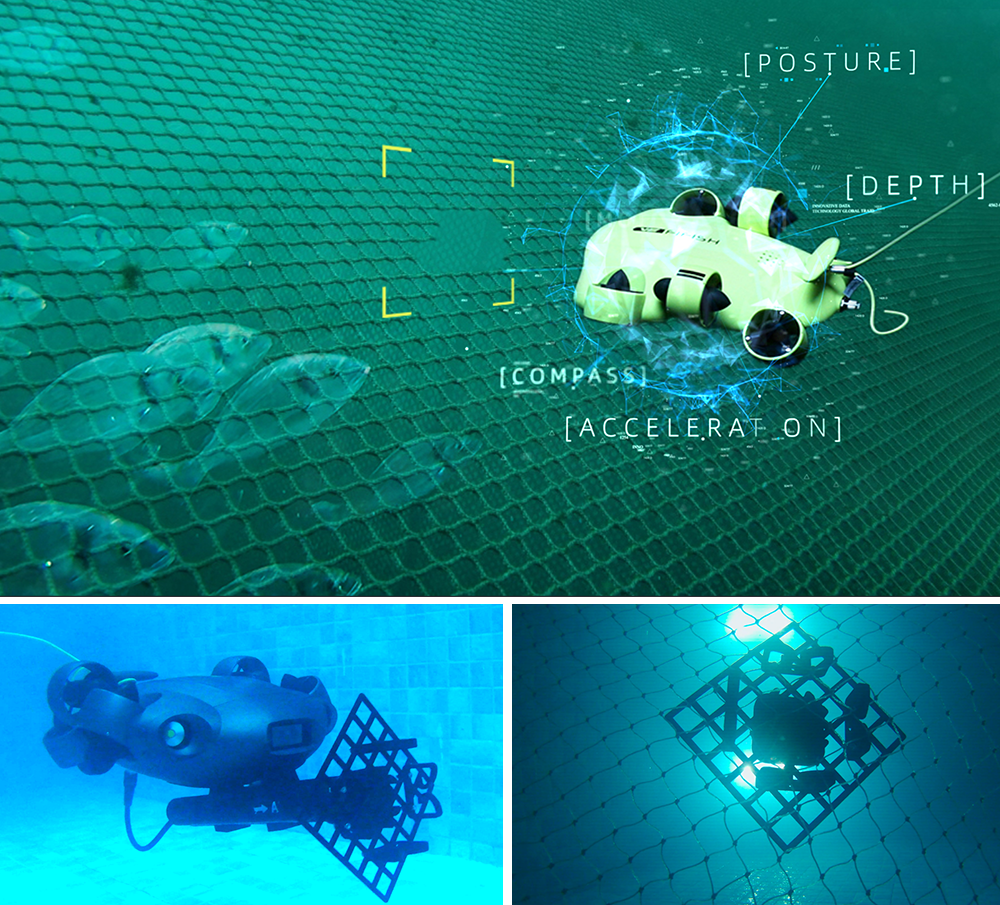
\includegraphics[height=3cm]{images/Qysea_1} &
    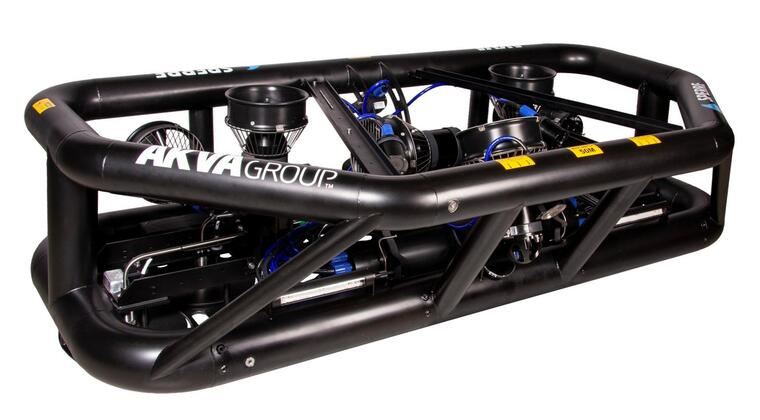
\includegraphics[height=2cm]{images/AKVA_1} &
    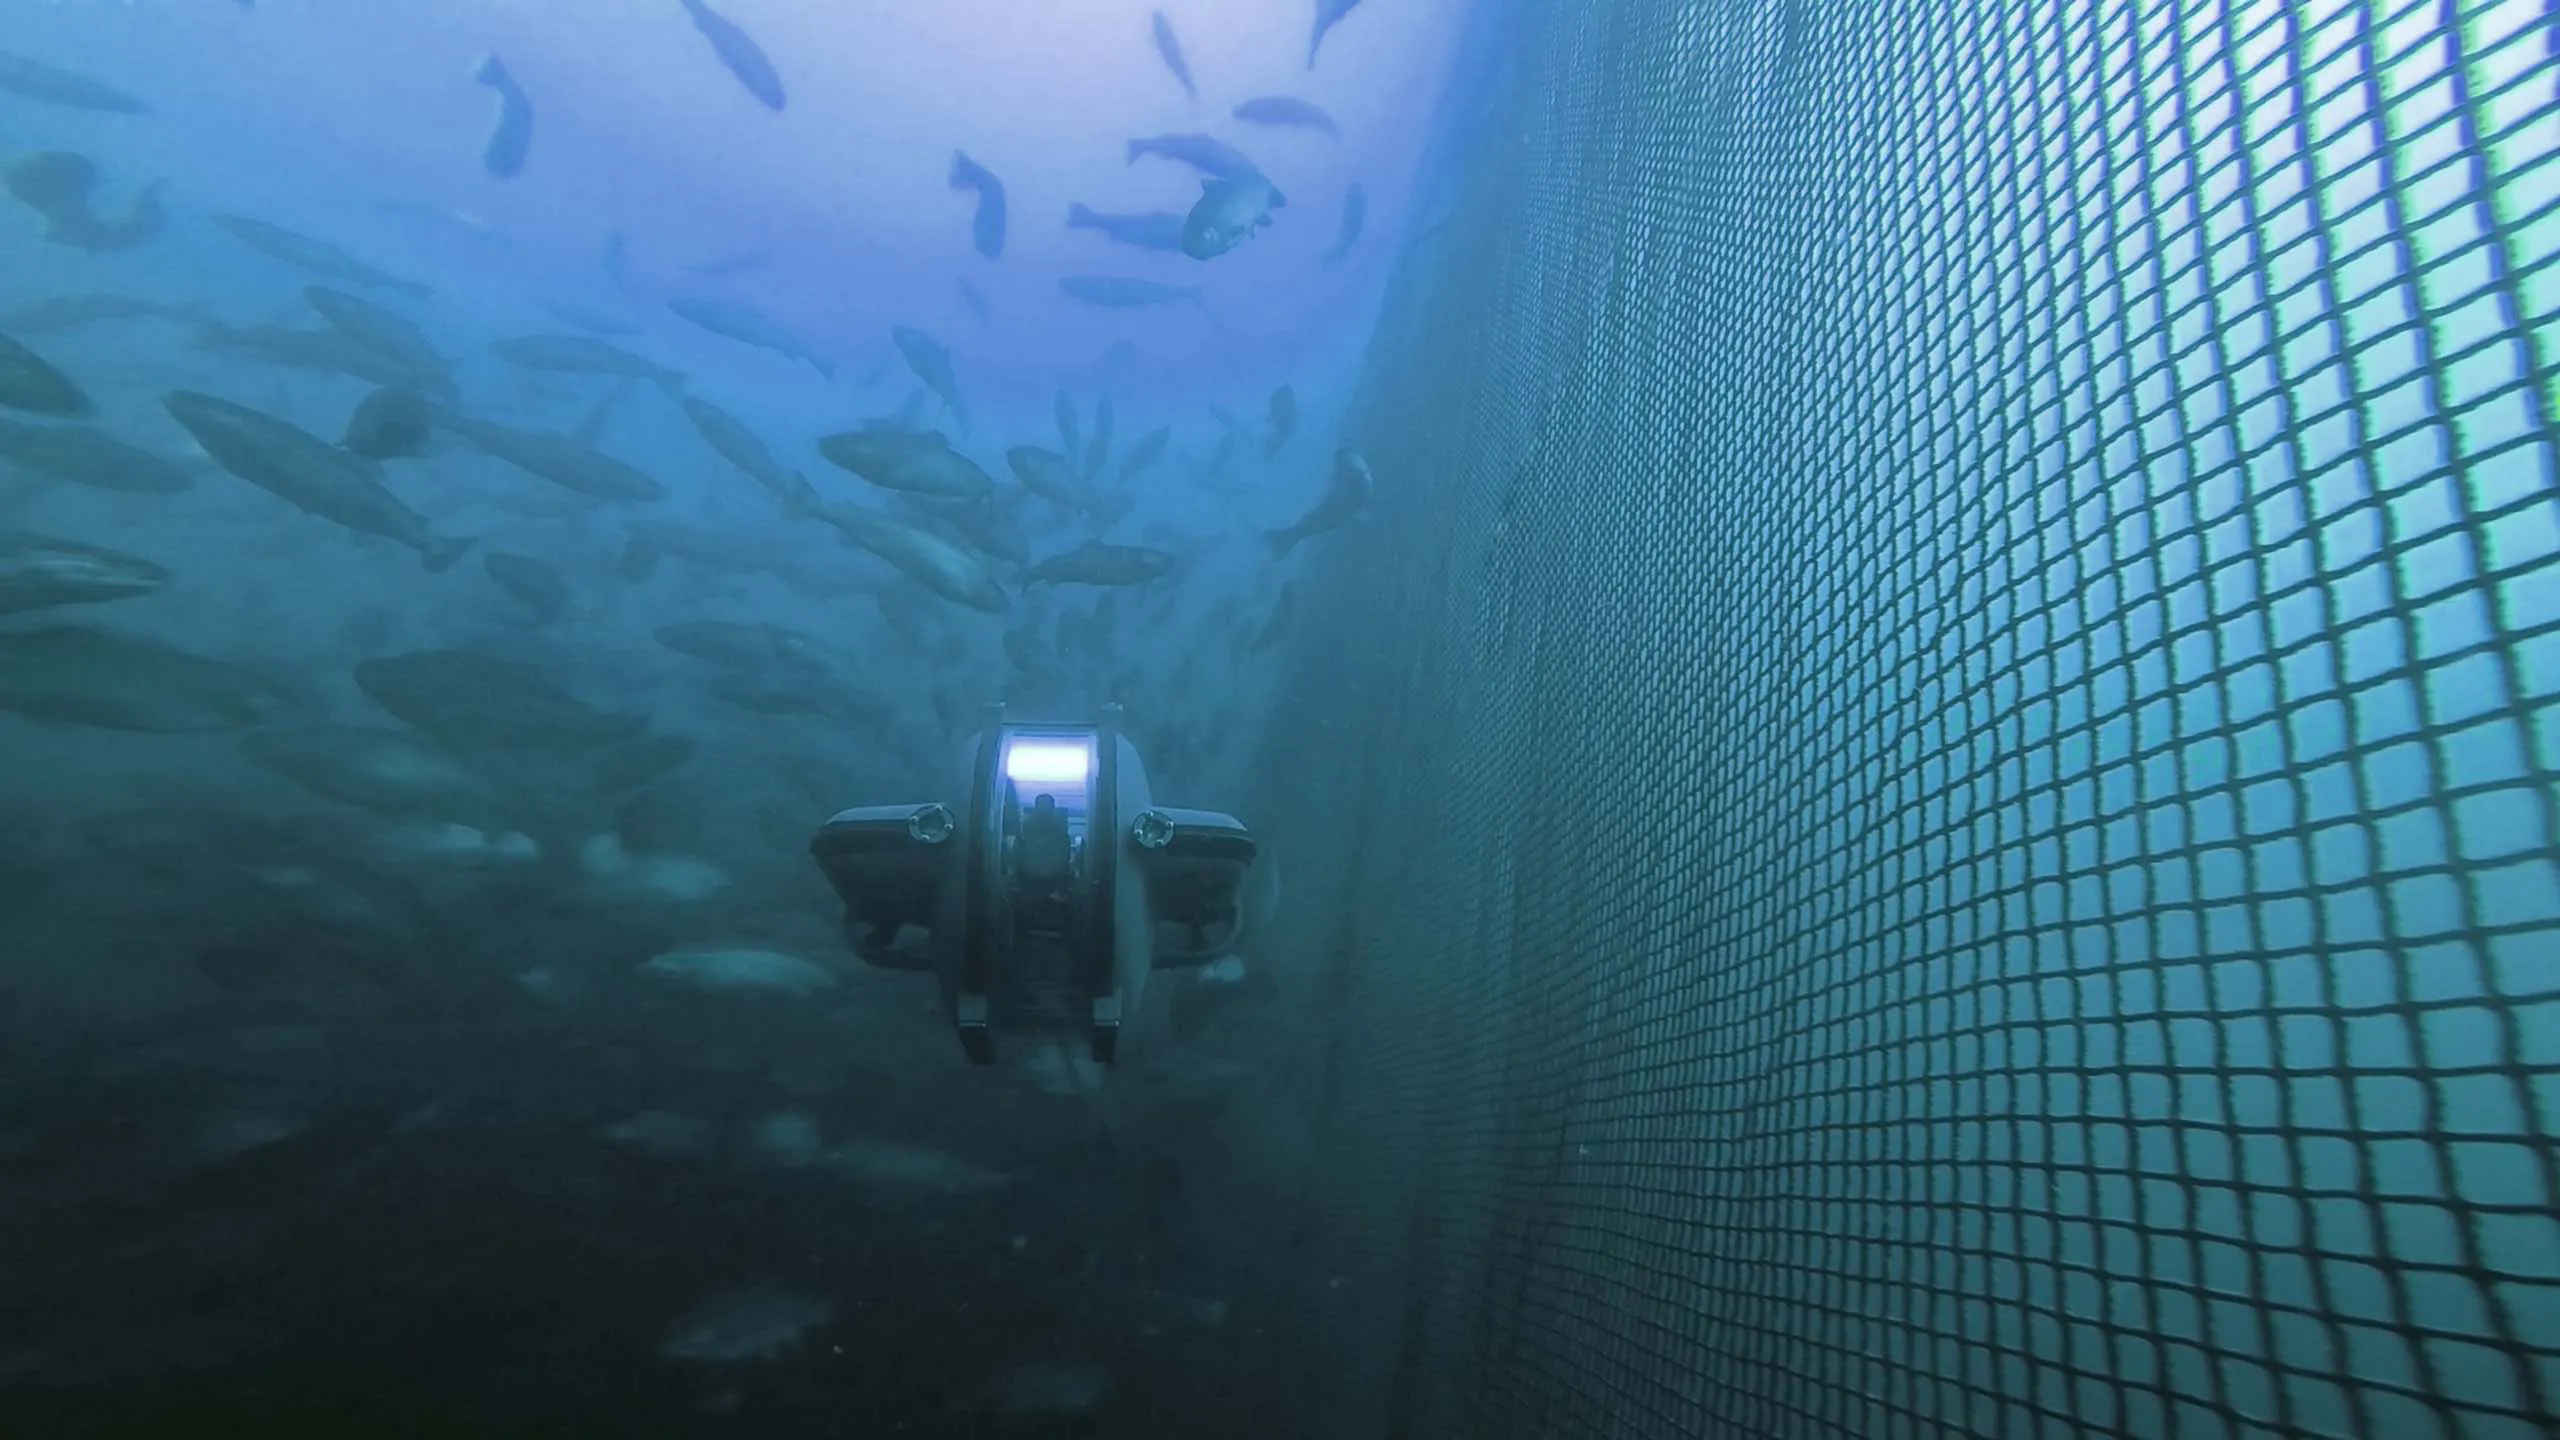
\includegraphics[height=3cm]{images/Deep_1} \\
    (a) & (b) & (c)
    \end{tabular}
    \caption{\label{fig:empresas_manual}(a)  ROV de Qysea para reparación de huecos en \cite{Qysea}. (b) Robot de AKVA para limpieza de redes en \cite{AKVAgroup}. (c)ROV de Deep Trekker para inspección manual de redes en  \cite{DeepTrekker}.}
    \end{center}
\end{figure}


En contraste con las empresas mencionadas, InnovaSea \cite{InnovaSea} ofrece un sistema completo conformado por distintos equipos entre las granjas que miden parámetros del agua, nivel de alimentación, comportamiento y salud del pescado. Posee un dispositivo entre las conexiones cada granja, controlando el sistema de amarre. Sin embargo, no ofrece una solución para la inspección de redes. Cabe resaltar que tampoco utiliza ROVs, mas sí dispositivos que, para otros parámetros, realiza mediciones de forma estática. Para análisis de estas mediciones, a comparación de las empresas anteriormente mencionadas, sí utilizan herramientas de visión computacional para obtener la biomasa del pescado, control de alimentación, entre otros. 

\begin{figure} [!h]
    \begin{center}
    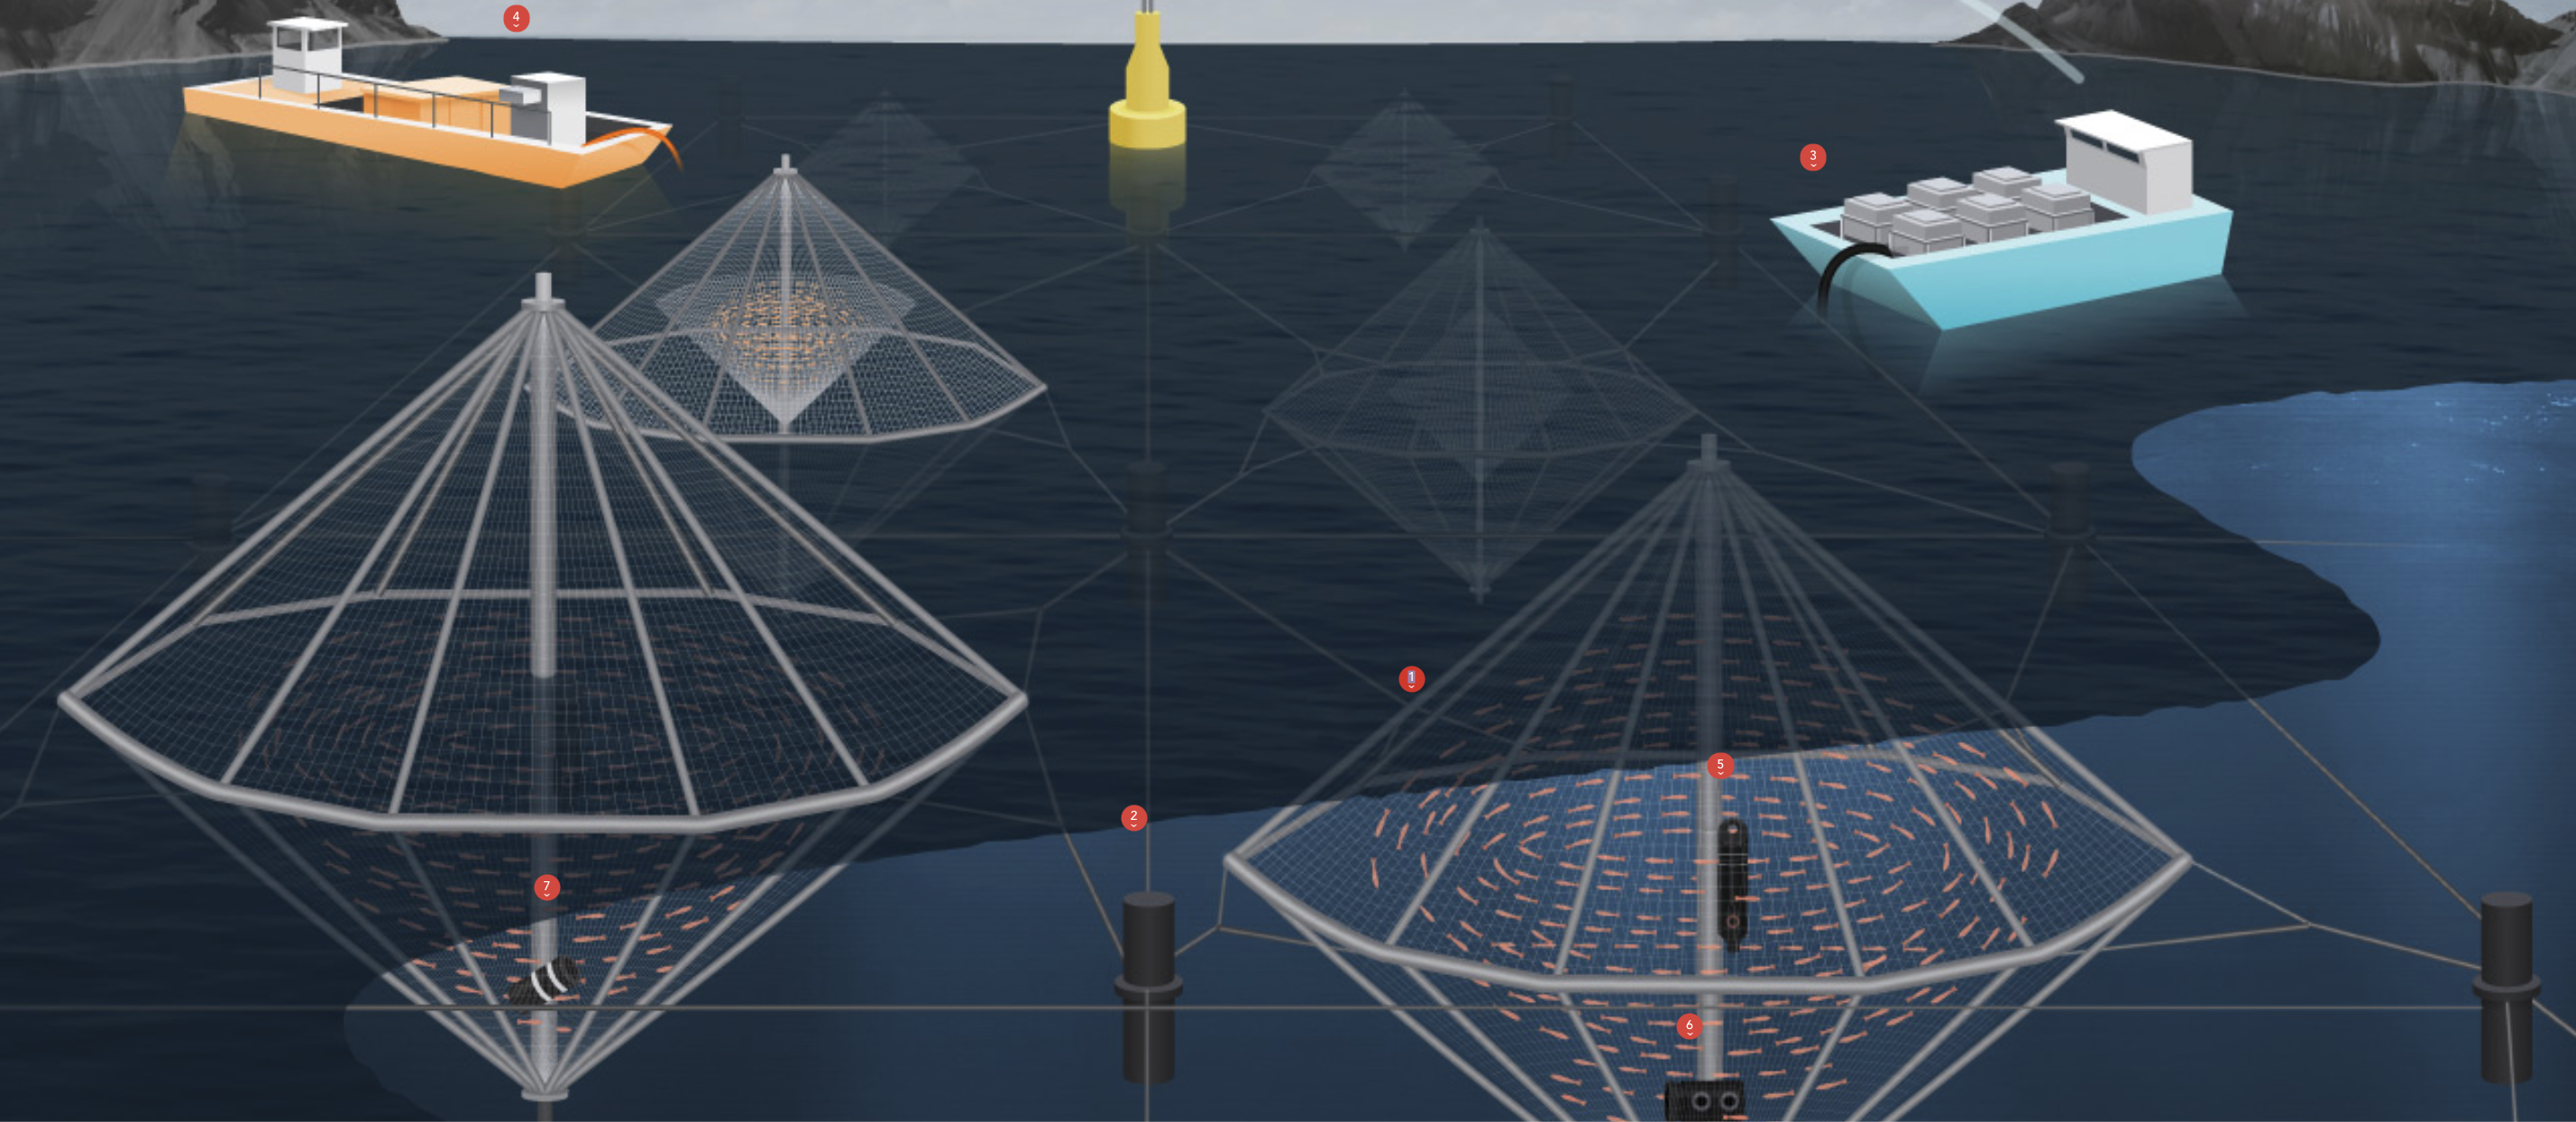
\includegraphics[height=4cm]{images/InnovaSea_1} 
    \caption{\label{fig:InnovaSea_sistema} Distribución de equipos de Innova Sea alrededor de las granjas de jaula en  \cite{InnovaSea}.}
    \end{center}
\end{figure}


\subsection{Limpieza de redes}
Empresas como Autobots, Watbots o Remora robotics desarrollan robots submarinos con instrumentos que quitan todo material en la red. Los 3 ofrecen una limpieza autónoma,  Watbots y Remora pueden detectar obstáculos y esquivarlos, y Watbots también detecta huecos \cite{Watbots}. Cabe resaltar que estos robots solo poseen un diseño para limpieza de redes, sin la capacidad de ser modular. Asimismo, las empresas se enfocan en realizar servicios en las redes, mas no en las demás partes de la granja. Por este motivo no se le puede agregar una garra para arreglar el hueco, o una cámara para observar el comportamiento del pescado. 


\section{Métodos de visión computacional}
Los métodos encontrados se basaron de documentos de investigación ya que las empresas no especifican qué utilizan. Muchos artículos comentan la reducción de tiempo en monitoreo de redes con el uso de sus algoritmos implementados en robots submarinos, mayormente ROVs. Frente a buzos para la inspección de redes, como el caso de \cite{cite:Betancourt}, disminuyó de 2 horas a 10 minutos. Sin embargo, aún es necesario la intervención de un piloto, ya que no se ha realizado aún una trayectoria autónoma del robot a usarse. El proceso puede separarse por uso de distintos sensores hidro-acústicos o procesamiento visual con el uso de cámaras. Dado que el objetivo de esta investigación está relacionado con visión computacional, se describirán aquellos procesos que usen cámaras.  

\subsection{Para detección de huecos}
Dado el patrón que se encuentra en las redes, dentro de las soluciones encontradas se usa mayormente procesamiento de imágenes digitales. Tal es el caso del artículo desarrollado por Betancourt \cite{cite:Betancourt}. En este se implementa un ROV que, dentro de varios servicios, detecta los agujeros de una red de forma autónoma y en tiempo real. El proceso parte con la partición del video por frames, donde se realiza un filtrado de la imagen de la red, obteniendo de resultado una imagen binaria utilizando el método de Otsu. Seguidamente, con la transformada de Hough se logra obtener las líneas de la red y la corrección de la imagen. Luego, con el algoritmo Convex hull obtienen la intersección de líneas representando los nudos y el área de cada 4 nudos con el uso de centroides. Finalmente, en este último algoritmo, se obtiene una representación del patrón de la red. En caso se presenten líneas que no tengan nodos, se entiende como un agujero. Se puede apreciar en la figura \ref{fig:Betancourt_1} el resultado de cada paso. 

\begin{figure}[!h]
    \begin{center}
    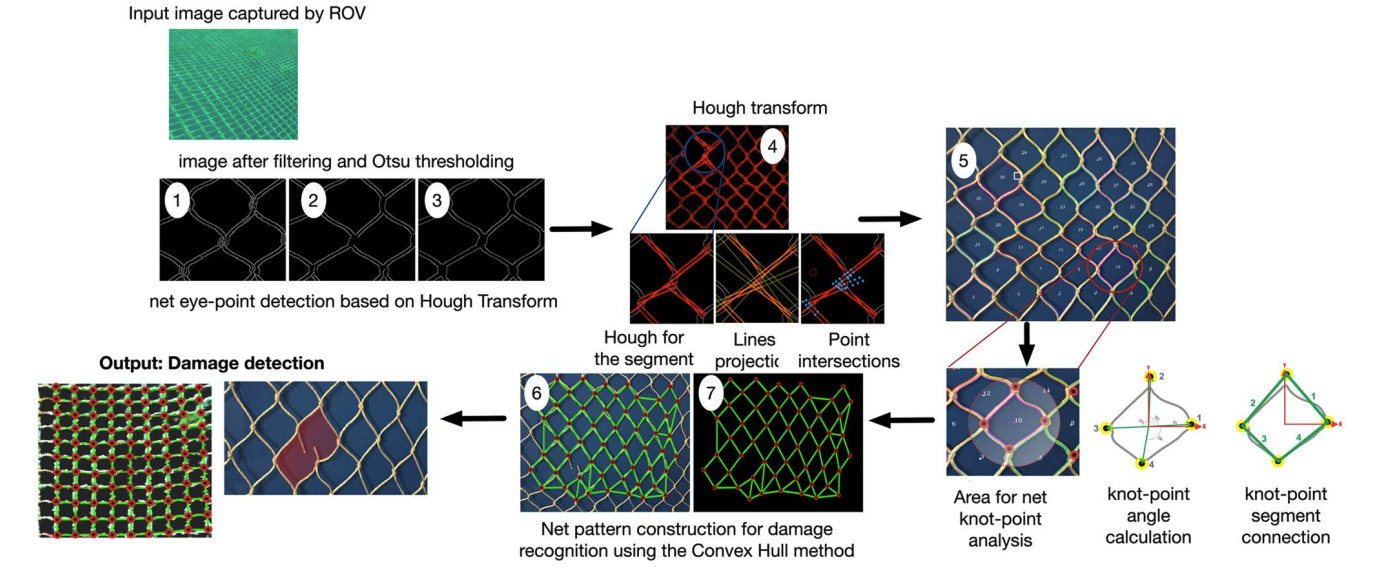
\includegraphics[height=6.2cm]{images/Betancourt_1} 
    \caption{\label{fig:Betancourt_1}Representación de todos los pasos de \cite{cite:Betancourt}.}
    \end{center}
\end{figure}

Dentro del hardware usado en \cite{cite:Betancourt}, se menciona el uso del ROV creado por OpenROV que tenía 1 cámara HD con 4 luces LEDs. Una de las desventajas de este algoritmo es que presenta un 79 \% de efectividad, donde era más efectivo en escenarios donde las imágenes de la red estaban perfectamente alineadas o tenían una perspectiva horizontal orientada a la izquierda. La precisión disminuyó en escenarios con perspectiva horizontal orientada a la derecha debido a problemas de calibración de la cámara y limitaciones del método de transformación de Hough. Esta efectividad se realizó en la implementación del algoritmo y robot en un represa en Colombia, mas no con el uso de un simulador. Cabe resaltar que no usan ningún método de Machine Learning o Deep Learning.

Al igual que este artículo, el procedimiento es realizado por Zhao \cite{cite:Zhao}, donde se segmenta la imagen para encontrar los nodos de la red y conectarlos. Sin embargo, la detección de nudos es distinta, ya que, a través de filtros, se encuentran las 4 esquina generadas por una esquina. Luego, para encontrar los huecos este realiza una medida de las áreas creadas por las líneas de la red. En este sentido, cuando se haya una área grande, se estima como un hueco. Asimismo, este artículo añade filtros que eliminan la suciedad, mejorando la selección de la red. Este proceso puede ser de ayuda no solo para eliminar la suciedad, sino para estimar a cuánto está y saber cuándo hacer limpieza de la red. Se puede apreciar en la figura \ref{fig:Zhao_1} el resultado de cada paso. 

\begin{figure} [!h]
    \begin{center}
    \begin{tabular}{cc}
    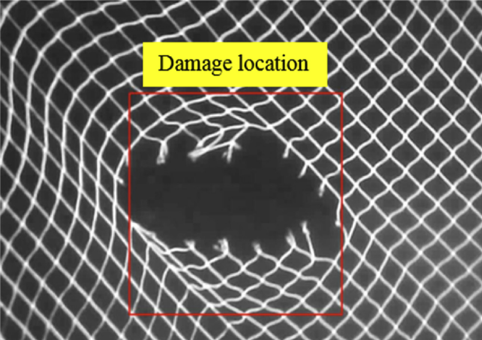
\includegraphics[height=3.5cm]{images/Zhao_11} &
    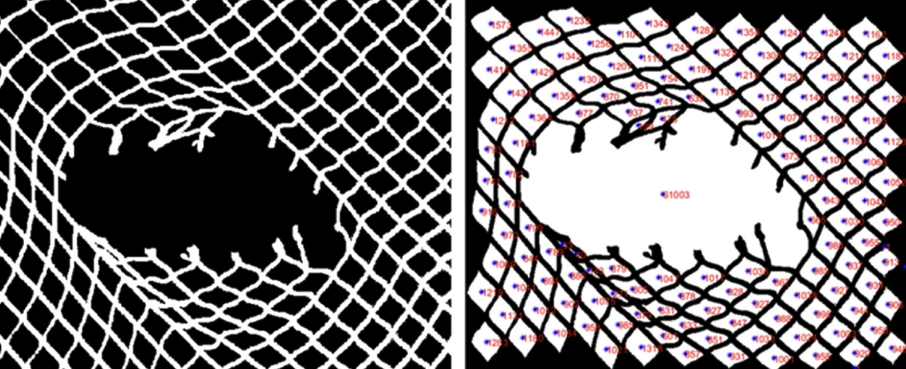
\includegraphics[height=3.5cm]{images/Zhao_12} \\
    \end{tabular}
    \caption{\label{fig:Zhao_1}Representación de la imagen de la red al ser segmentada y al detectar los huecos en \cite{cite:Zhao}.}
    \end{center}
\end{figure}

Para la implementación de este algoritmo se menciona el uso de una cámara con resolución 1920 × 1040. Al igual que en \cite{cite:Betancourt}, no usó un simulador, sino pruebas in situ. Del igual, no se ve la presencia de Machine o Deep Learning. A comparación de \cite{cite:Betancourt}, este algoritmo, en función al área encontrada como hueco en la red, crea un histograma de gradientes de features y obtiene picos locales de la curva que permiten estimar una posición del hueco. 

Por otro lado, dado que las redes tienen distintos patrones y el color del agua varia geográficamente, el uso de Deep Learning es más robusto que procesamiento de imágenes. Según Zhang \cite{cite:Zhang} se puede realizar directamente una combinación de redes convolucionales con algoritmos que logran obtener una probabilidad alta de detección de huecos. El algoritmo propone la revisión de la red en tiempo real aplicando Para un mejor entendimiento del algoritmo se muestra en la imagen \ref{fig:Zhang_1}.

\begin{figure}[!h]
    \begin{center}
    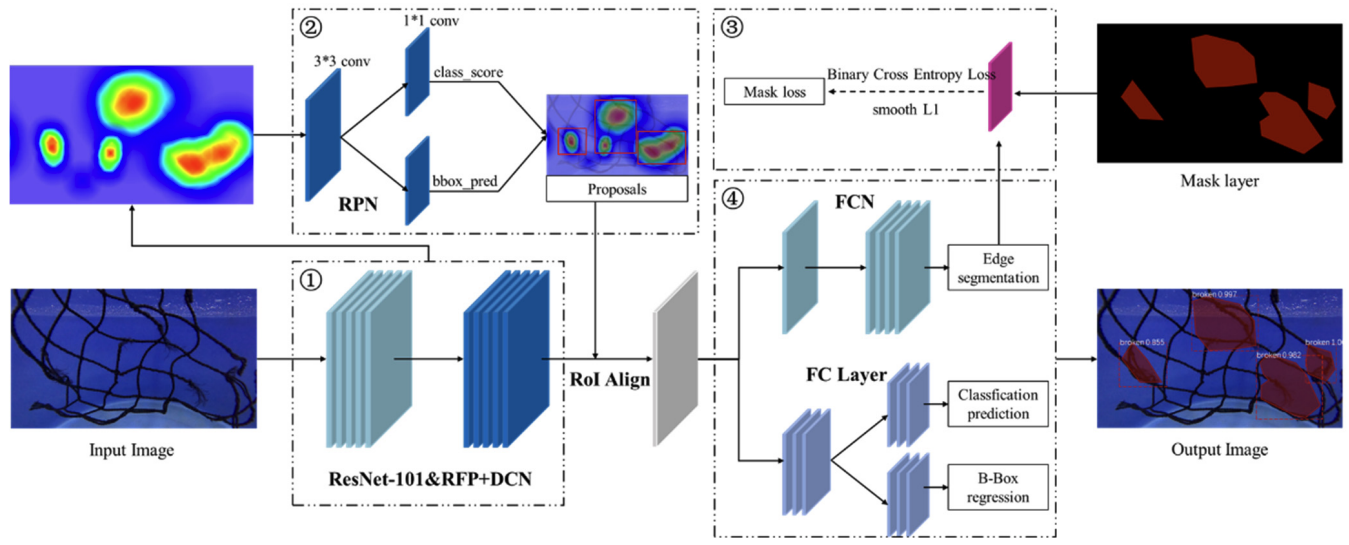
\includegraphics[height=6cm]{images/Zhang_1} 
    \caption{\label{fig:Zhang_1}Representación de todos los pasos de \cite{cite:Zhang}. 1 indica el backbone para la extracción de características, 2 indica la red de propuesta de región, 3 indica la rama de entrenamiento de segmentación de borde y 4 indica el módulo de clasificación y detección de objetos.}
    \end{center}
\end{figure}


La prueba del algoritmo hecho en \cite{cite:Zhang} se realiza en una piscina con una red dañada junto a una GoPro con resolución de 5312x2988 pixeles. Con la prueba de distintos modelos de redes neuronales, como se aprecia en la figura \ref{tab:Zhang}, se obtuvo una efectividad del 94.48 \%. Como comparación, se tiene un 15.48 \% mayor de efectividad que el algoritmo de \cite{cite:Betancourt} usando procesamiento de imágenes. 
\begin{table}[h!]
    \centering
    \begin{tabular}{ccccc}
        Model & Missing Rate & AP & F1 Score & FPS \\
        \hline
        Mask R-CNN & 28.56\% & 86.62\% & 85.81\% &  4.46 \\
        Mask R-CNN+RFP & 11.18\% & 90.12\% & 89.27\% & 4.20 \\
        Mask R-CNN+DCN & 21.83\% & 91.90\% & 90.11\% & 4.82 \\
        Mask R-CNN+RFP+DCN & 7.12\% & 94.48\% & 94.02\% & 4.74 \\
        \hline
    \end{tabular}
    \caption{La detección de daños en diferentes modelos neuronales mejorados en \cite{cite:Zhang}.}
    \label{tab:Zhang}
\end{table}



Finalmente, se ha buscado métodos de visión computacional que complementan los procesos actuales explicados anteriormente. Tal es el caso del uso de reconstrucción 3D, el cual puede complementar al reconocimiento en tiempo real de las redes, sino saber con mayor exactitud dónde se encuentran los huecos y los puntos con mayor suciedad. Esto es posible con un método de mapeo y localización llamado 'Inertial Visual SLAM' realizada por Ferrera \cite{cite:Ferrera}. Para 


Un punto a resaltar como algoritmos que necesitan de un robot para ser validados es el uso de simuladores. Gran parte de las investigaciones encontradas no realizan simulaciones. Esto es ya que mayormente tienen un ROV con el que se puede realizar pruebas directamente de redes en uso o en ambientes controlados. 



% la Fig. \ref{fig:diagram2}, y es importante recordar la relación mostrada en \eqref{eq:1}.


% \begin{figure} 
% \begin{center}
% \begin{tabular}{cc}
% 
\includegraphics[height=3cm]{images/logo_utec.png} &
% 
\includegraphics[height=2cm]{images/logo_utec.png} \\
% (a) & (b)
% \end{tabular}
% \caption{\label{fig:diagram2} . (a) Logo en tamaño de 3 centímetros. (b) Logo en tamaño de 2 centímetros.}
% \end{center}
% \end{figure}

% \begin{table}[H]
%     \centering
%     \begin{tabular}{c|c}
%         Tiempo($s$) & Distancia($m$) \\
%         \hline
%         10 & 23 \\
%         20 & 33 \\
%         30 & 43 \\
%         40 & 53 \\
%     \end{tabular}
%     \caption{Tiempos versus distancia.}
%     \label{tab:tiempo_versus_distancia}
% \end{table}


% \cite{Reumann2012}.
%
% \begin{equation}
%   \label{eq:1}
%   a+b=\sqrt{\frac{4}{3}},
% \end{equation}
% donde $a$ y $b$ son escalares.
